\section{市场方案}
\subsection{市场需求调研方式}

企业与市场的关系是不可分割的。简单来说:企业是为了市场的需要而存在的,也可以说企业是服务于市场的;市场有着不同的需求,而企业为了满足市场的种种需求而发展壮大。在进行新产品暨课程开发前,本公司将充分做好市场需求调研,在考虑公司今后长远发展规划的基础之上寻求需求最大最具市场价值的发展方向,这一方面应该后期将专门由公司知识管理部负责。注意调研的有效性及专业性,可参考的一些方式:

\paragraph{大数据调研}\

从易观、艾瑞等专业大数据平台或其他方面获取数据,分析目前市场状况及未来发展趋势并作出市场发展判断,从而选定新课程研发方向。

\paragraph{线下调研}\

通过对线下机构及线上用户的需求调研,根据调研结果有针对性地开展接下来的产品研发方向选择工作。此方法能有效增强与用户的交互性并且获得数据更为直接可靠。

\paragraph{知识管理规划}\

依据公司战略发展目标,与具体可实施性,在与课程运营部密切合作沟通的同时,把握前沿知识管理与知识创造的方法,同时按照公司知识管理方法指导实施,协助修正市场调研得出的课程研发方向。

\subsection{市场需求预调研}
如图\ref{fg:B2B2C2017}:
\begin{figure}[H]
	\centering
	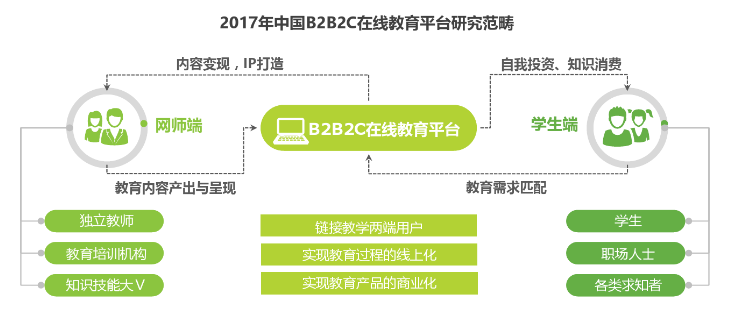
\includegraphics[width=0.9\columnwidth]{figures/B2B2C2017.png}
	%  \setlength{\abovecaptionskip}{0pt}
	%  \setlength{\belowcaptionskip}{-20pt}
	\caption{2017年中国B2B2C在线教育平台研究范畴}
	\label{fg:B2B2C2017}
\end{figure}

\paragraph{知识提供方}\

知识变现的需要,特别是受过高等教育的人,他们会有很多隐性知识的储备,但没有渠道输出,没有可以获得利益的渠道。或者他们有这样的渠道,但是收到的效果并不好。

\paragraph{知识需求方}\

知识改变命运,现代人对终身教育的需要,不断学习的理念的深入人心,对个人技能的补充,对大学所学专业内容的不适应,对深入学习的需要。

\begin{figure}[H]
	\centering
	
\includegraphics[width=0.9\columnwidth]{figures/relationship}
	%  \setlength{\abovecaptionskip}{0pt}
	%  \setlength{\belowcaptionskip}{-20pt}
	\caption{两者的关系}
	\label{fg:relationship}
\end{figure}


\subsection{销售模式}

\subsubsection{前期}\

寻找校园代理,通过校园代理来拓宽教师来源渠道,在系统开发的同时,进行课程的录制,课程录制的方向是:先进行市场调查,市场调查的依据是询问线下教育行业人士,然后针对性的进行课程录制,课程销售交给线下教育行业人士,通过获得收益分成的方式吸引合作者。

\begin{figure}[H]
	\centering
	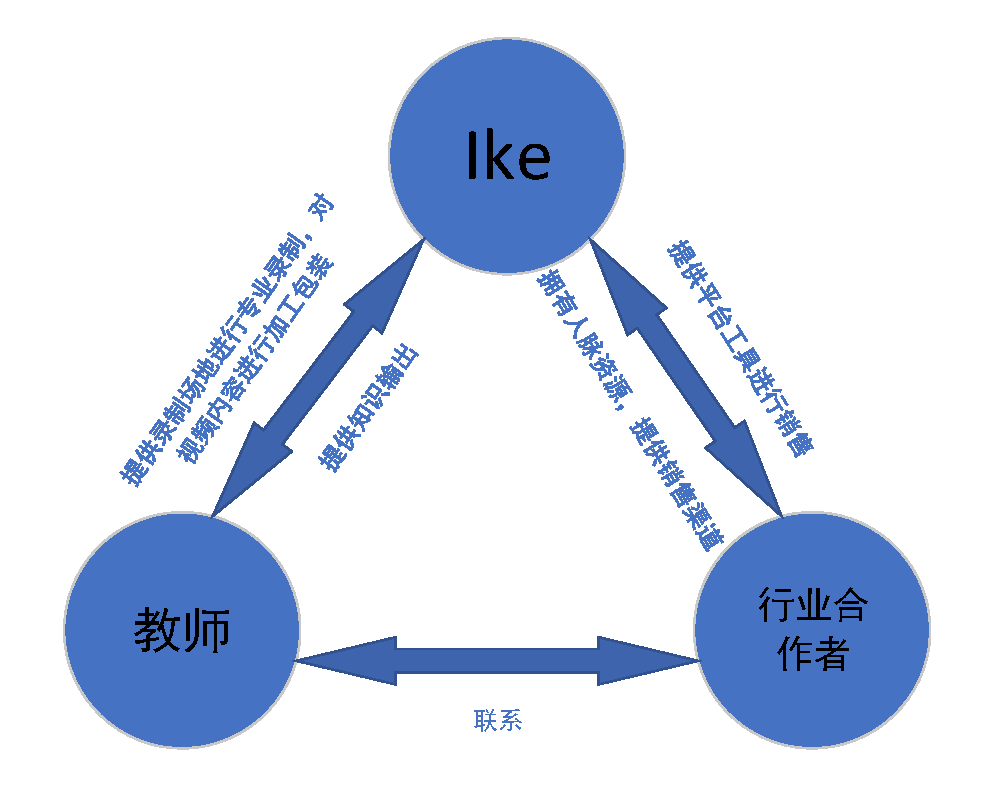
\includegraphics[width=0.9\columnwidth]{figures/partnership}
	%  \setlength{\abovecaptionskip}{0pt}
	%  \setlength{\belowcaptionskip}{-20pt}
	\caption{合作关系}
	\label{fg:partnership}
\end{figure}

\subsubsection{中期}\

当前期盈利模式获得一定收益之后,增加销售部,销售部组成人员主要来源于社会招聘,通过市场上的有经验的销售人员,通过销售人员来留住客户,同时,课程录制开始逐渐完善平台总体课程框架,开始录制大学专业介绍,初步拥有品牌知名度;对平台课程视频资源的重新整合加工,二次销售给市场,加大融资。部分课程免费开放吸引流量打开市场。

\subsubsection{后期}\

独立营业模式超过现有的教育平台,有足够强壮的基础课程体系后,进军K12领域并寻求与地方政府的合作,通过低价格的形式将课程卖给或者送给偏远贫困地区学生,打响平台品牌;与电商合作;增加知识管理部门,对平台已有的三大知识储存载体,进行知识的提炼,知识元的加工,转化的二次加工产品输出,公司主要盈利和影响力将来源于此。

\subsection{产品定价}

产品定价是产品在市场中占据主动的前提,适当的产品定价能帮助企业在激烈的市场竞争中占得先机。本公司运营产品目前主要为课程成品,定价时主要考虑课程的内容价值以及目前在线教育市场的供求关系,在兼顾消费者的购买力基础之上,通过一定算法得出产品最适宜的市场定价。目前针对公司运营时期变化主要采取三种定价方式。

\subsubsection{质量加成定价}\

课程研发之初,本公司将充分考虑课程知识、教师水平、内容难获取程度等多发面因素确保产品质量。产品定价时,在考虑目前市场价的基础之上,针对本产品的质量优势进行一定的加权处理,同时综合考虑教师知名度、教师背景、教师形象等可能对课程销售产生影响的因素,最终确定本课程定价。

\subsubsection{市场导向定价}\

在课程销售经过一定时间之后,参考市场销售反馈情况,课程的定价需要根据市场反馈作出一定调整。初步考虑将产品的浏览量与购买量的比值关系作为市场反馈的一个表现因素,根据市场导向最终确定课程的定价调整计划。

\subsubsection{竞争导向定价}\

在课程销售的后期,考虑同类型企业将会越来越多出现,市场竞争也将会越来越激烈。激烈的市场竞争之中要想取得优势就需要看清形势,针对当前同类产品竞争情况作出针对性价格调整,以在竞争中保持优势地位。




